\documentclass[dvipsnames]{beamer}

\usepackage[utf8]{inputenc}
\usepackage{fancybox}
\usepackage{environ,fancyvrb}

\usepackage{tikz}

\newcommand{\ds}{\displaystyle}
\newcommand{\grad}{\nabla}
\newcommand{\ih}{\boldsymbol{\hat{\textbf{\i}}}}
\newcommand{\jh}{\boldsymbol{\hat{\textbf{\j}}}}
\newcommand{\vF}{\boldsymbol{\vec{\textbf{F}}}}


\beamertemplatenavigationsymbolsempty

\title{4.4 Nonhomogeneous equations: \\ method of undetermined coefficients}

\subtitle{a lecture for MATH F302 Differential Equations}

\author{Ed Bueler, Dept.~of Mathematics and Statistics, UAF}

\date{Fall 2023}


\usetheme{Pittsburgh}


\begin{document}

\setbeamertemplate{itemize item}{$\bullet$}
\setbeamertemplate{itemize subitem}{$\circ$}


\begin{frame}
\titlepage

\centerline{\tiny for textbook: \, D. Zill, \emph{A First Course in Differential Equations with Modeling Applications}, 11th ed.}
\end{frame}


\begin{frame}{general solutions to nonhomogeneous DEs}

\begin{itemize}
\item for an $n$th-order, linear, and nonhomogeneous DE
\begin{equation*}
    a_n(x) y^{(n)} + a_{n-1}(x) y^{(n-1)} + \dots + a_1(x) y' + a_0(x) y \stackrel{\ast}{=} g(x)
\end{equation*}
\item \dots the general solution is a sum of the general solution of the associated \emph{homogeneous} equation
\begin{equation*}
    a_n(x) y^{(n)} + a_{n-1}(x) y^{(n-1)} + \dots + a_1(x) y' + a_0(x) y = 0
\end{equation*}
plus one \emph{particular solution} $y_p(x)$ of $\ast$
    \begin{itemize}
    \item the general solution of the homogeneous equation is called the \emph{complementary function} $y_c(x)$
    \end{itemize}

\bigskip
\item main structure: \alert{$y(x) = y_c(x) + y_p(x)$ solves $\ast$}
\end{itemize}
\end{frame}


\begin{frame}{example 1}

\begin{itemize}
\item \emph{example 1}: find the general solution:
    $$y'' + 4 y = e^{-x}$$
\end{itemize}

\vspace{60mm}
\end{frame}


\begin{frame}{example 1, cont.}

\begin{itemize}
\item verify that $y(x) = c_1 \cos 2x + c_2 \sin 2x + \frac{1}{5} e^{-x}$ solves
    $$y'' + 4 y = e^{-x}$$

\vspace{60mm}
\end{itemize}
\end{frame}


\begin{frame}{example 1, cont.$^2$}

\begin{itemize}
\item solve the initial value problem:
    $$y'' + 4 y = e^{-x}, \qquad y(0)=-1, \quad y'(0)=1$$

\vspace{60mm}
\end{itemize}
\end{frame}


\begin{frame}{example 2}

\begin{itemize}
\item the idea of ``undetermined coefficients'' is to \alert{try $y_p(x)$ which has the same general form as the nonhomogeneity $g(x)$}
\item \emph{example 2 ($\approx$ \#5 in 4.4)}: find the general solution:
    $$y'' + 4 y' + 4y = x^2 - 2 x \hspace{50mm}$$
\end{itemize}

\vspace{50mm}
\end{frame}


\begin{frame}{example 3}

\begin{itemize}
\item \emph{example 3 (\#8 in 4.4)}: find the general solution:
    $$4 y'' - 4 y' - 3 y = \cos 2x \hspace{50mm}$$
\end{itemize}

\vspace{60mm}
\end{frame}


\begin{frame}{trial forms for the particular solution}

\begin{itemize}
\item we need some guidance on how to guess!
\item in words:

\begin{quotation}
\noindent \alert{For $y_p$ try a linear combination of all linearly-independent functions generated by repeated differentiation of $g(x)$.}
\end{quotation}

\vspace{-3mm}
\item as a table:
\end{itemize}

\hfill 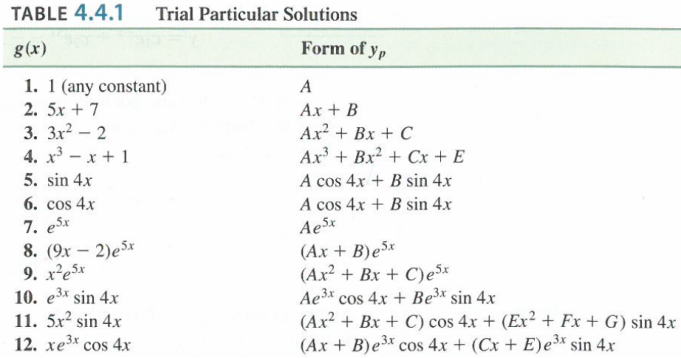
\includegraphics[width=0.8\textwidth]{figs/yptable}
\end{frame}


\begin{frame}{example 4 \emph{shows we still have issues!}}

\begin{itemize}
\item \emph{example 4 ($\approx$ \#13 in 4.4)}: find the general solution:
    $$y'' + 9 y = 2 \cos 3x \hspace{50mm}$$
\end{itemize}

\vspace{60mm}
\end{frame}


\begin{frame}{guidance on the hard case}

\begin{itemize}
\item the problematic case happens when our guess for $y_p$ ``accidently'' contain terms which also appear in $y_c$
    \begin{itemize}
    \item because the left side then annihilates those terms
    \item \dots which blocks us from determining $y_p$
    \end{itemize}

\bigskip
\item guidance in words:

\begin{quotation}
\noindent \alert{If the trial form of $y_p$ contains terms that duplicate terms in $y_c$ then multiply the trial form by $x^n$ where $n$ is the smallest power that eliminates the duplication.}
\end{quotation}
\end{itemize}
\end{frame}


\begin{frame}{example 5}

\begin{itemize}
\item \emph{example 5 (\#29 in 4.4)}: solve the initial value problem:
    $$5 y'' + y' = -6 x, \qquad y(0) = 0, \quad y'(0)=-10$$
\end{itemize}

\vspace{60mm}
\end{frame}


\begin{frame}{example 6}

\begin{itemize}
\item \emph{example 6 (\#32 in 4.4)}: solve the initial value problem:
    $$y'' - y = \cosh x, \qquad y(0) = 2, \quad y'(0)=12$$
\end{itemize}

\vspace{60mm}
\end{frame}


\begin{frame}{example 6, cont.}

\begin{itemize}
\item the last slide had an impressive calculation, so we should \dots
\item verify that $y(x)=7 e^x - 5 e^{-x} + \frac{1}{4} x e^x - \frac{1}{4} x e^{-x}$ solves\, $y'' - y = \cosh x,\, y(0) = 2, y'(0)=12$
\end{itemize}

\vspace{55mm}
\end{frame}


\begin{frame}{clearly}

\begin{itemize}
\item clearly \alert{you} need to practice examples, not just me
\end{itemize}
\end{frame}


\begin{frame}{what we are skipping next}

we are \alert{skipping} the following sections:
\begin{itemize}
\item \S 4.5 \emph{Undetermined Coefficients---Annihilator Approach}

a more abstract view of undetermined coefficients \dots but no more powerful than our superposition method
\item \S 4.6 \emph{Variation of parameters}

a general approach to nonhomogeneous linear equations \underline{but} one may not be able to compute the integrals you get
    \begin{itemize}
    \item it is somewhat like reduction of order in \S 4.2
    \end{itemize}
\item \S 4.7 \emph{Cauchy-Euler equations}

another class of homogeneous differential equations which can be solved via an auxiliary equation
\item \S 4.8 \emph{Green's Functions}

mostly relevant to boundary value problems (not in Math 302)
\item \S 4.9 \emph{Solving Systems of Linear DEs by Elimination}

a way of solving systems \dots which are important \dots but done generally and powerfully in chapter 8
\end{itemize}
\end{frame}



\begin{frame}{expectations}

to learn this material, just listening to a lecture is \emph{not} enough
     \begin{itemize}
     \item \emph{read} section 4.4 in the textbook
     \item do Homework 4.4
     \item find YouTube worked examples; search ``nonhomogeneous differential equations'' and ``method of undetermined coefficients''
     \end{itemize}
\end{frame}

\end{document}

